\documentclass{standalone}
\usepackage{tikz}
\usetikzlibrary{patterns, positioning}

\begin{document}
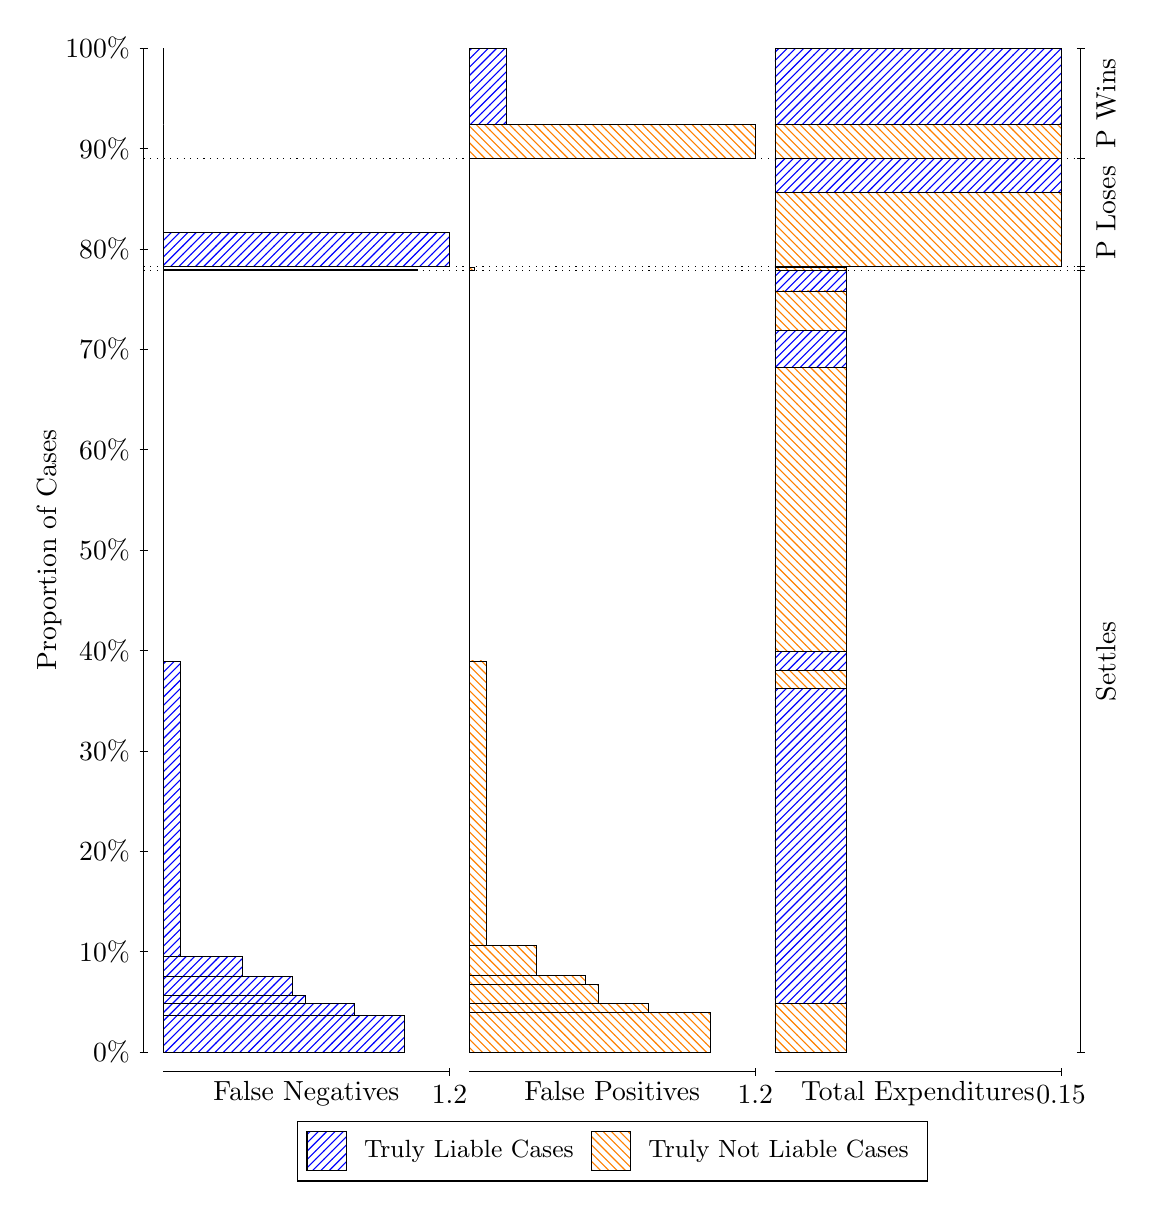
\begin{tikzpicture}
\draw[black, very thin] (1.5,1.75) -- (1.5,14.5);
\node[rotate=90, anchor=center] at (0.3, 8.125) {Proportion of Cases};
\draw[black, very thin] (1.45,1.75) -- (1.55,1.75);
\node[anchor=east] at (1.45, 1.75) {0\%};
\draw[black, very thin] (1.45,3.025) -- (1.55,3.025);
\node[anchor=east] at (1.45, 3.025) {10\%};
\draw[black, very thin] (1.45,4.3) -- (1.55,4.3);
\node[anchor=east] at (1.45, 4.3) {20\%};
\draw[black, very thin] (1.45,5.575) -- (1.55,5.575);
\node[anchor=east] at (1.45, 5.575) {30\%};
\draw[black, very thin] (1.45,6.85) -- (1.55,6.85);
\node[anchor=east] at (1.45, 6.85) {40\%};
\draw[black, very thin] (1.45,8.125) -- (1.55,8.125);
\node[anchor=east] at (1.45, 8.125) {50\%};
\draw[black, very thin] (1.45,9.4) -- (1.55,9.4);
\node[anchor=east] at (1.45, 9.4) {60\%};
\draw[black, very thin] (1.45,10.675) -- (1.55,10.675);
\node[anchor=east] at (1.45, 10.675) {70\%};
\draw[black, very thin] (1.45,11.95) -- (1.55,11.95);
\node[anchor=east] at (1.45, 11.95) {80\%};
\draw[black, very thin] (1.45,13.225) -- (1.55,13.225);
\node[anchor=east] at (1.45, 13.225) {90\%};
\draw[black, very thin] (1.45,14.5) -- (1.55,14.5);
\node[anchor=east] at (1.45, 14.5) {100\%};

\draw[black, very thin] (13.4,1.75) -- (13.4,14.5);
\draw[black, very thin] (13.35,1.75) -- (13.45,1.75);
\node[anchor=west] at (13.35, 1.75) {};
\draw[black, very thin] (13.35,11.673) -- (13.45,11.673);
\node[anchor=west] at (13.35, 11.673) {};
\draw[black, very thin] (13.35,11.724) -- (13.45,11.724);
\node[anchor=west] at (13.35, 11.724) {};
\draw[black, very thin] (13.35,13.094) -- (13.45,13.094);
\node[anchor=west] at (13.35, 13.094) {};
\draw[black, very thin] (13.35,14.5) -- (13.45,14.5);
\node[anchor=west] at (13.35, 14.5) {};

\draw[black, very thin, pattern color=blue, pattern=north east lines] (1.75,1.75) rectangle (4.8107,2.2146);
\draw[black, very thin, pattern color=blue, pattern=north east lines] (1.75,2.2146) rectangle (4.1788,2.3678);
\draw[black, very thin, pattern color=blue, pattern=north east lines] (1.75,2.3678) rectangle (3.5469,2.4712);
\draw[black, very thin, pattern color=blue, pattern=north east lines] (1.75,2.4712) rectangle (3.3889,2.7088);
\draw[black, very thin, pattern color=blue, pattern=north east lines] (1.75,2.7088) rectangle (2.7571,2.9682);
\draw[black, very thin, pattern color=blue, pattern=north east lines] (1.75,2.9682) rectangle (1.9672,6.7061);
\draw[black, very thin, pattern color=orange, pattern=north west lines] (1.75,6.7061) rectangle (1.75,11.673);
\draw[black, very thin, pattern color=blue, pattern=north east lines] (1.75,11.673) rectangle (4.9687,11.686);
\draw[black, very thin, pattern color=orange, pattern=north west lines] (1.75,11.686) rectangle (1.75,11.724);
\draw[black, very thin, pattern color=blue, pattern=north east lines] (1.75,11.724) rectangle (5.3833,12.156);
\draw[black, very thin, pattern color=orange, pattern=north west lines] (1.75,12.156) rectangle (1.75,13.094);
\draw[black, very thin, pattern color=orange, pattern=north west lines] (1.75,13.094) rectangle (1.75,13.526);
\draw[black, very thin, pattern color=blue, pattern=north east lines] (1.75,13.526) rectangle (1.75,14.5);
\draw[black, very thin, pattern color=orange, pattern=north west lines] (5.6333,1.75) rectangle (8.694,2.2518);
\draw[black, very thin, pattern color=orange, pattern=north west lines] (5.6333,2.2518) rectangle (7.9042,2.3678);
\draw[black, very thin, pattern color=orange, pattern=north west lines] (5.6333,2.3678) rectangle (7.2723,2.6054);
\draw[black, very thin, pattern color=orange, pattern=north west lines] (5.6333,2.6054) rectangle (7.1143,2.7192);
\draw[black, very thin, pattern color=orange, pattern=north west lines] (5.6333,2.7192) rectangle (6.4824,3.108);
\draw[black, very thin, pattern color=orange, pattern=north west lines] (5.6333,3.108) rectangle (5.8505,6.7167);
\draw[black, very thin, pattern color=blue, pattern=north east lines] (5.6333,6.7167) rectangle (5.6333,11.673);
\draw[black, very thin, pattern color=orange, pattern=north west lines] (5.6333,11.673) rectangle (5.6926,11.711);
\draw[black, very thin, pattern color=blue, pattern=north east lines] (5.6333,11.711) rectangle (5.6333,11.724);
\draw[black, very thin, pattern color=orange, pattern=north west lines] (5.6333,11.724) rectangle (5.6333,12.662);
\draw[black, very thin, pattern color=blue, pattern=north east lines] (5.6333,12.662) rectangle (5.6333,13.094);
\draw[black, very thin, pattern color=orange, pattern=north west lines] (5.6333,13.094) rectangle (9.2667,13.526);
\draw[black, very thin, pattern color=blue, pattern=north east lines] (5.6333,13.526) rectangle (6.1072,14.5);
\draw[black, very thin, pattern color=orange, pattern=north west lines] (9.5167,1.75) rectangle (10.425,2.3678);
\draw[black, very thin, pattern color=blue, pattern=north east lines] (9.5167,2.3678) rectangle (10.425,6.3652);
\draw[black, very thin, pattern color=orange, pattern=north west lines] (9.5167,6.3652) rectangle (10.425,6.6027);
\draw[black, very thin, pattern color=blue, pattern=north east lines] (9.5167,6.6027) rectangle (10.425,6.8403);
\draw[black, very thin, pattern color=orange, pattern=north west lines] (9.5167,6.8403) rectangle (10.425,10.449);
\draw[black, very thin, pattern color=blue, pattern=north east lines] (9.5167,10.449) rectangle (10.425,10.914);
\draw[black, very thin, pattern color=orange, pattern=north west lines] (9.5167,10.914) rectangle (10.425,11.416);
\draw[black, very thin, pattern color=blue, pattern=north east lines] (9.5167,11.416) rectangle (10.425,11.673);
\draw[black, very thin, pattern color=orange, pattern=north west lines] (9.5167,11.673) rectangle (10.425,11.711);
\draw[black, very thin, pattern color=blue, pattern=north east lines] (9.5167,11.711) rectangle (10.425,11.724);
\draw[black, very thin, pattern color=orange, pattern=north west lines] (9.5167,11.724) rectangle (13.15,12.662);
\draw[black, very thin, pattern color=blue, pattern=north east lines] (9.5167,12.662) rectangle (13.15,13.094);
\draw[black, very thin, pattern color=orange, pattern=north west lines] (9.5167,13.094) rectangle (13.15,13.526);
\draw[black, very thin, pattern color=blue, pattern=north east lines] (9.5167,13.526) rectangle (13.15,14.5);
\draw[black, dotted] (1.5,11.673) -- (13.4,11.673);
\draw[black, dotted] (1.5,11.724) -- (13.4,11.724);
\draw[black, dotted] (1.5,13.094) -- (13.4,13.094);
\draw[black, very thin] (1.75,1.5) -- (5.3833,1.5);
\node[anchor=north] at (3.5667, 1.5) {False Negatives};
\draw[black, very thin] (5.3833,1.45) -- (5.3833,1.55);
\node[anchor=north] at (5.3833, 1.45) {1.2};

\draw[black, very thin] (5.6333,1.5) -- (9.2667,1.5);
\node[anchor=north] at (7.45, 1.5) {False Positives};
\draw[black, very thin] (9.2667,1.45) -- (9.2667,1.55);
\node[anchor=north] at (9.2667, 1.45) {1.2};

\draw[black, very thin] (9.5167,1.5) -- (13.15,1.5);
\node[anchor=north] at (11.333, 1.5) {Total Expenditures};
\draw[black, very thin] (13.15,1.45) -- (13.15,1.55);
\node[anchor=north] at (13.15, 1.45) {0.15};

\node[black, centered, rotate=90] at (13.72, 6.7114) {Settles};

\node[black, centered, rotate=90] at (13.72, 12.409) {P Loses};
\node[black, centered, rotate=90] at (13.72, 13.797) {P Wins};

\draw (7.449999999999999,1.5) node[draw=none] (baseCoordinate) {};
\begin{scope}[align=center]
        \matrix[scale=0.5, draw=black, below=0.5cm of baseCoordinate, nodes={draw}, column sep=0.1cm]{
            \node[rectangle, draw, minimum width=0.5cm, minimum height=0.5cm, pattern=north east lines, pattern color=blue] {}; &
            \node[draw=none, font=\small] (B) {Truly Liable Cases}; &
            \node[rectangle, draw, minimum width=0.5cm, minimum height=0.5cm, pattern=north west lines, pattern color=orange] {}; &
            \node[draw=none, font=\small] (B) {Truly Not Liable Cases}; \\
            };
\end{scope}

\end{tikzpicture}
\end{document}